% !TeX root = ../final.tex
% Revised one-hour lecture script.
% Teaching arc: LET THE SYSTEM DECIDE.

\chapter{From automated experimentation to self-driving chemistry}

\begin{notebox}
  \keypoint{What do you need to learn from this chapter?}
  By the end of this chapter, you should be able to distinguish fixed experimental design, sequential selection, automation, programmability, and autonomy.
  You should understand how a surrogate model and acquisition function turn completed measurements into new experimental choices, how exploration and exploitation compete, and why multiobjective optimisation, quality control, safe recovery, and human-defined constraints are part of a self-driving laboratory.
\end{notebox}

% Suggested timing: 0--7 min
\section{When does an experimental campaign become adaptive?}

In Chapter~7, a robot could execute hundreds of experiments from a design chosen before the campaign began.
Even if every liquid transfer, temperature profile, measurement, and data-processing step is automated, the scientific decisions may remain fixed.

A sequential campaign is different.
After one experiment or batch has been measured, the result changes which experiment is selected next.
The loop is

\solution{4.5cm}{%
  \centering
  define objective $\longrightarrow$ select experiment $\longrightarrow$ execute\\[0.6em]
  $\longrightarrow$ measure and validate $\longrightarrow$ update model or state\\[0.6em]
  $\longrightarrow$ select the next experiment
}

Sequential does not necessarily mean one reaction at a time.
A batch can be selected when reactions run in parallel or when analytical scheduling dominates the cost.
The trade-off is that all experiments in a batch are selected before the outcomes of their neighbours are known.

Before any outcomes exist, a space-filling or representative design can be a sensible way to initialise the campaign.
It chooses experiments for coverage.
After responses have been measured, the best next experiment may instead be selected because it is predicted to improve the objective, reduce relevant uncertainty, or test a suspected boundary.
Coverage and adaptive selection therefore answer different questions.

\solution{3.8cm}{%
  \textbf{Add the missing arrow.} Take the fixed HTE workflow from Chapter~7 and draw the feedback arrow that turns it into an adaptive campaign.\\[0.5em]
  What information must cross that arrow? A validated response, its quality status, the updated state of knowledge, and the next executable action.
}

A stopping rule is also a decision.
The campaign might stop when it reaches a target, exhausts a budget, shows little expected improvement, covers the relevant domain, or encounters a safety or hardware constraint.
Without a stopping rule, ``optimise'' is not a complete instruction.

% Suggested timing: 7--18 min
\section{Choosing the next experiment}

An optimisation problem begins with variables, an objective, constraints, an experimental budget, and a stopping rule.
Continuous variables include temperature, time, concentration, pressure, flow rate, and equivalents.
Categorical variables include solvent, base, catalyst, ligand, and reactor configuration.
The complete combinatorial space is reduced by solubility, compatibility, equipment limits, safety, and material availability.

The objective defines improvement.
Highest analytical yield, highest isolated yield, highest selectivity, maximum productivity, minimum process mass intensity, lowest cost, and lowest hazard are different objectives.
An optimiser does not discover what we value; it follows the quantity we encode.

\solution{4.0cm}{%
  \textbf{Write an optimisation problem for one reaction.}
  \begin{itemize}
    \item variables and allowed ranges;
    \item categorical choices;
    \item objective with units;
    \item hard constraints;
    \item experimental budget;
    \item stopping rule.
  \end{itemize}
}

A surrogate model approximates the expensive experimental response using the observations collected so far.
A Gaussian-process model is conceptually useful because it returns both a mean prediction and an uncertainty estimate over the defined search space.
Uncertainty tends to be lower near informative observations and larger in poorly sampled regions.
It is conditional on the model, representation, and noise assumptions.
It does not guarantee that an unrepresented mechanism, phase change, or analytical failure has been considered.

An acquisition function ranks candidate experiments using the surrogate model.
Pure exploitation selects the condition with the best predicted response.
Pure exploration selects an uncertain condition that could improve the model.
Expected improvement and related acquisition functions balance those motives.

\begin{figure}[htbp]
  \centering
  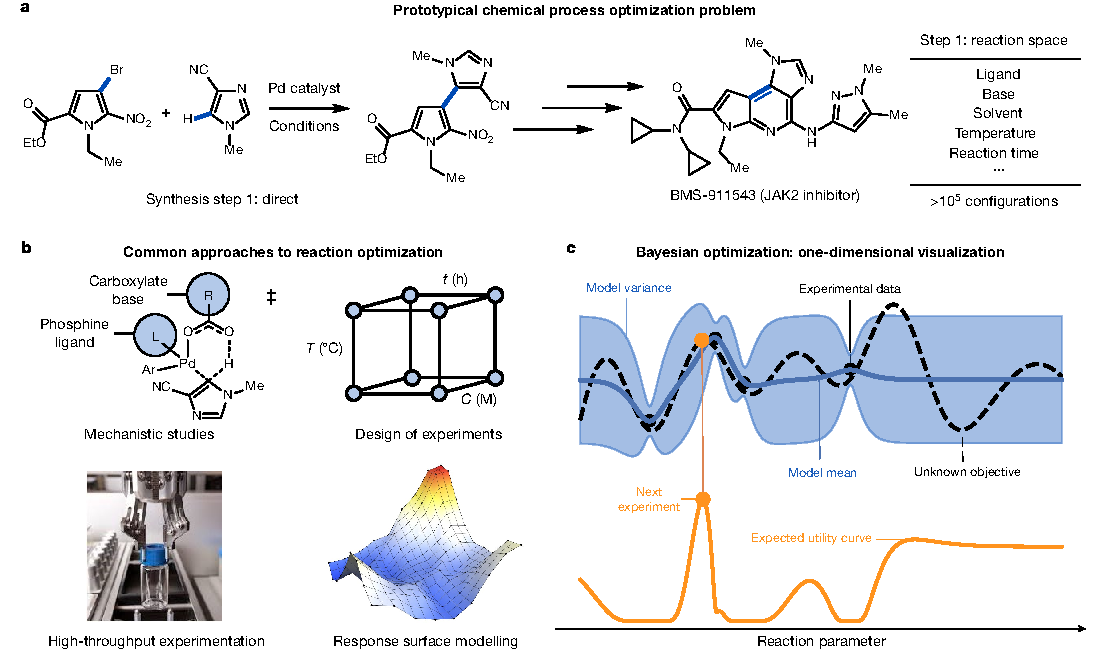
\includegraphics[width=\textwidth,height=0.58\textheight,keepaspectratio]{figures/chapter08-autonomise/01-shields-bayesian-optimisation-concept-fig1.pdf}
  \caption{Bayesian reaction optimisation as a sequential experimental loop, contrasted with conventional optimisation strategies. Reproduced from Shields \textit{et al.}, \textit{Nature} (2021), Fig.~1.}
  \label{fig8-shields-concept}
\end{figure}

\solution{4.2cm}{%
  \textbf{Turn the published overview into the decision loop used in this chapter.}
  \begin{itemize}
    \item Number selection, execution, measurement, model update, and reselection.
    \item Mark what is supplied by the chemist before the first experiment.
    \item Mark what changes only after a validated outcome is returned.
  \end{itemize}
}

\solution{5.2cm}{%
  \textbf{Annotate a one-dimensional surrogate plot.}
  \begin{itemize}
    \item draw observed experiments;
    \item draw the predicted mean and uncertainty band;
    \item mark the current best result;
    \item mark an exploitative candidate with high predicted value and low uncertainty;
    \item mark an exploratory candidate with moderate predicted value and high uncertainty;
    \item sketch an acquisition function and select the next experiment.
  \end{itemize}
}

The acquisition function does not execute chemistry.
It assigns priorities inside the candidate space it has been given.
If the space contains unsafe or physically impossible conditions, those should be excluded or constrained rather than made attractive by high uncertainty.

\begin{figure}[htbp]
  \centering
  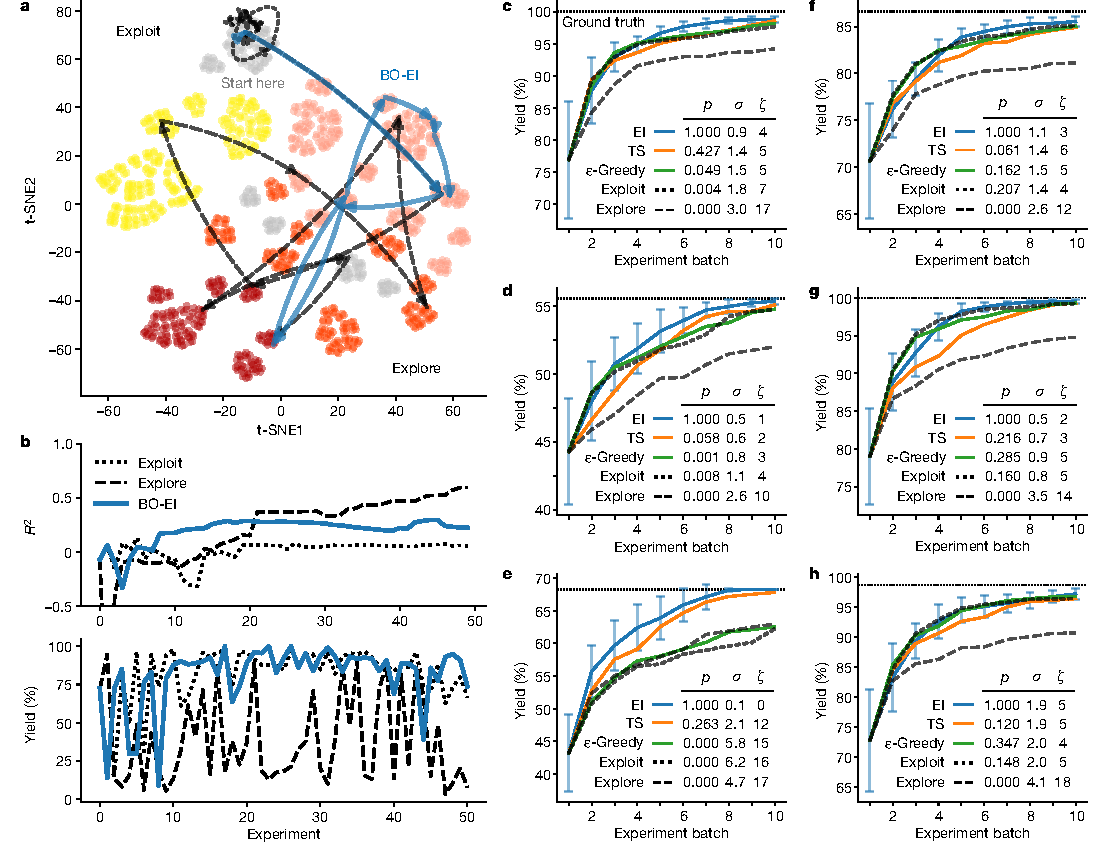
\includegraphics[width=\textwidth,height=0.65\textheight,keepaspectratio]{figures/chapter08-autonomise/02-shields-exploration-exploitation-fig3.pdf}
  \caption{Exploration, exploitation, and Bayesian optimisation choosing different experiments in a chemical search space. Reproduced from Shields \textit{et al.}, \textit{Nature} (2021), Fig.~3.}
  \label{fig8-shields-explore}
\end{figure}

\solution{4.0cm}{%
  \textbf{Explain three choices on the same search map.}
  \begin{itemize}
    \item Label one exploitative point and one exploratory point.
    \item Trace the Bayesian sequence and mark where new data change the next decision.
    \item Shade a chemically forbidden region that the acquisition function must never enter.
  \end{itemize}
}

\begin{warningbox}
  \keypoint{Model uncertainty is not permission to run an experiment.}
  Safety, compatibility, equipment, and material constraints define the delegated experimental space before acquisition values are compared.
\end{warningbox}

% Suggested timing: 18--26 min
\section{Bayesian optimisation in reaction development}

Shields and co-workers developed and benchmarked Bayesian reaction optimisation for synthetic chemistry using literature-derived datasets, a large experimental benchmark for palladium-catalysed direct arylation, and real optimisation campaigns.\mcite{Shields2021}
The study is particularly useful because it compared machine recommendations with human decisions under a fixed budget.

In the online game, participants had a simulated month to optimise a reaction and could run one batch of five reactions per workday.
Each choice returned the outcome of a real experiment from the complete high-throughput dataset.
Humans made better first choices than random initialisation on average, reflecting chemical experience.
Within three batches of five experiments, however, the average Bayesian optimiser had surpassed average human performance.
The optimiser also showed greater consistency across repeated runs and reached greater than $99\%$ yield in every run within the stated budget.

\begin{figure}[htbp]
  \centering
  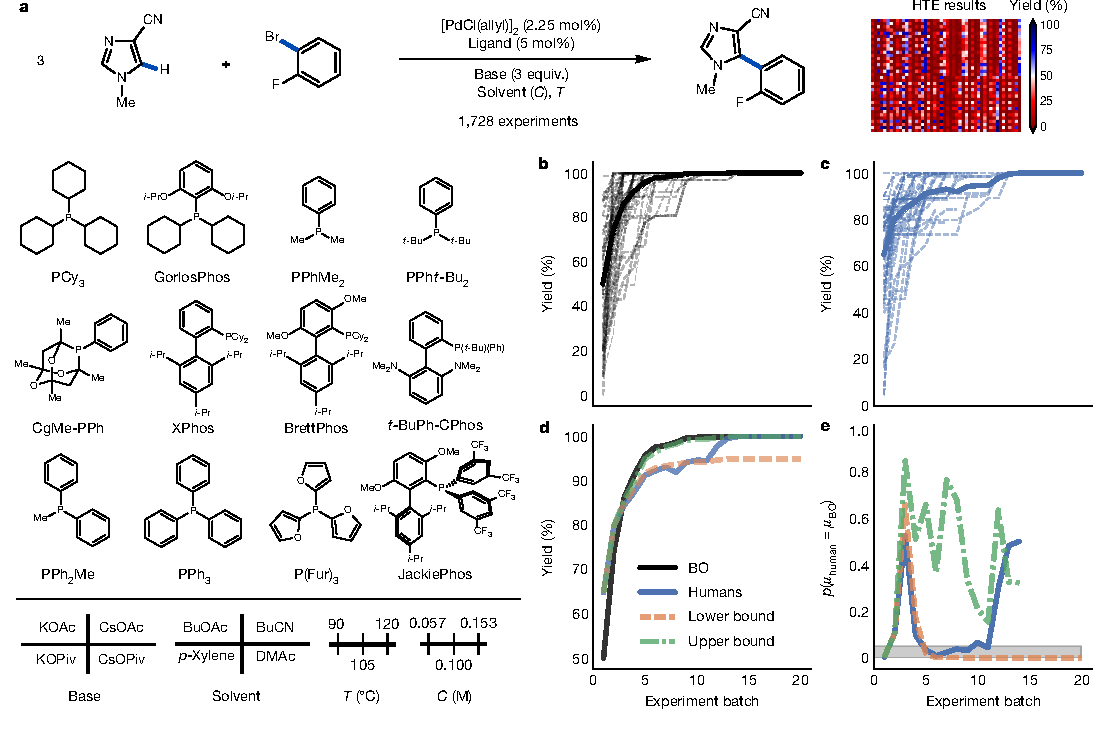
\includegraphics[width=\textwidth,height=0.60\textheight,keepaspectratio]{figures/chapter08-autonomise/03-shields-human-vs-bo-fig4.pdf}
  \caption{Direct-arylation benchmark and comparison of Bayesian and human optimisation under a fixed experimental budget. Reproduced from Shields \textit{et al.}, \textit{Nature} (2021), Fig.~4.}
  \label{fig8-shields-benchmark}
\end{figure}

\solution{4.4cm}{%
  \textbf{Annotate the benchmark plot.}
  \begin{itemize}
    \item mark the advantage of human chemical intuition in the first batch;
    \item mark the point at which average machine performance overtakes the human average;
    \item compare the spread of outcomes, not only the best run;
    \item identify the fixed experimental budget.
  \end{itemize}
}

The lesson is not that a machine is universally a better chemist.
The optimiser is unusually good at a bounded task: selecting combinations from a defined search space to improve a specified response using a consistent dataset.
Humans define the reaction, variables, encodings, constraints, analytical response, and success criterion.

The study also shows why batching matters.
Selecting five experiments in parallel is operationally efficient, but later experiments in the batch cannot respond to the earlier outcomes.
A laboratory must balance decision frequency against reaction and analytical throughput.

% Suggested timing: 26--32 min
\section{Several objectives and no universal optimum}

Chemical optimisation often contains competing objectives.
A condition with the highest yield may use a hazardous solvent, produce excessive waste, or have low throughput.
If one condition is at least as good as another in every objective and better in at least one, it dominates the other condition.
The non-dominated solutions form a Pareto front.

\solution{5.0cm}{%
  \textbf{Draw yield against process mass intensity or productivity.}
  \begin{itemize}
    \item mark several dominated points;
    \item draw the Pareto front;
    \item choose one point if yield is prioritised;
    \item choose another if waste or productivity is prioritised;
    \item add a forbidden region representing a safety constraint.
  \end{itemize}
}

The Pareto front exposes trade-offs; it does not decide among them.
A chemist or process team must still decide whether a small gain in yield justifies additional waste, cost, energy, or hazard.
Multiobjective optimisation therefore makes value judgements visible rather than eliminating them.

% Suggested timing: 32--39 min
\section{Automation, programmability, and autonomy}

These terms describe different relationships between a chemical procedure, hardware, measurements, and decisions.

\subsection{Automation executes a predefined procedure}

Merrifield and Stewart's automated peptide synthesiser mechanised the repeated deprotection, washing, coupling, and washing operations of solid-phase peptide synthesis.\mcite{Merrifield1965}
Reliable repetition transformed a demanding manual sequence into a scalable synthetic operation.
The machine did not measure the growing peptide and decide which amino acid should be added next.
The sequence and operating logic were supplied in advance.
It is therefore a clear example of automation without autonomy.

\subsection{Programmability represents and transfers a procedure}

The Chemputer developed by Steiner and co-workers represented organic synthesis through programmable unit operations.\mcite{Steiner2019}
A written procedure was translated into chemical code and combined with a graph describing the physical platform.
The resulting instructions controlled pumps, valves, heaters, separators, filters, and evaporators.
Reported syntheses of diphenhydramine, rufinamide, and sildenafil showed that reaction, work-up, isolation, and purification could be represented in an executable workflow.

The central advance is programmability: the logical procedure can be stored, edited, versioned, and compiled for compatible hardware.
The target and sequence remain specified by the chemist.
Code is not autonomy merely because it replaces manual instructions.

\begin{figure}[htbp]
  \centering
  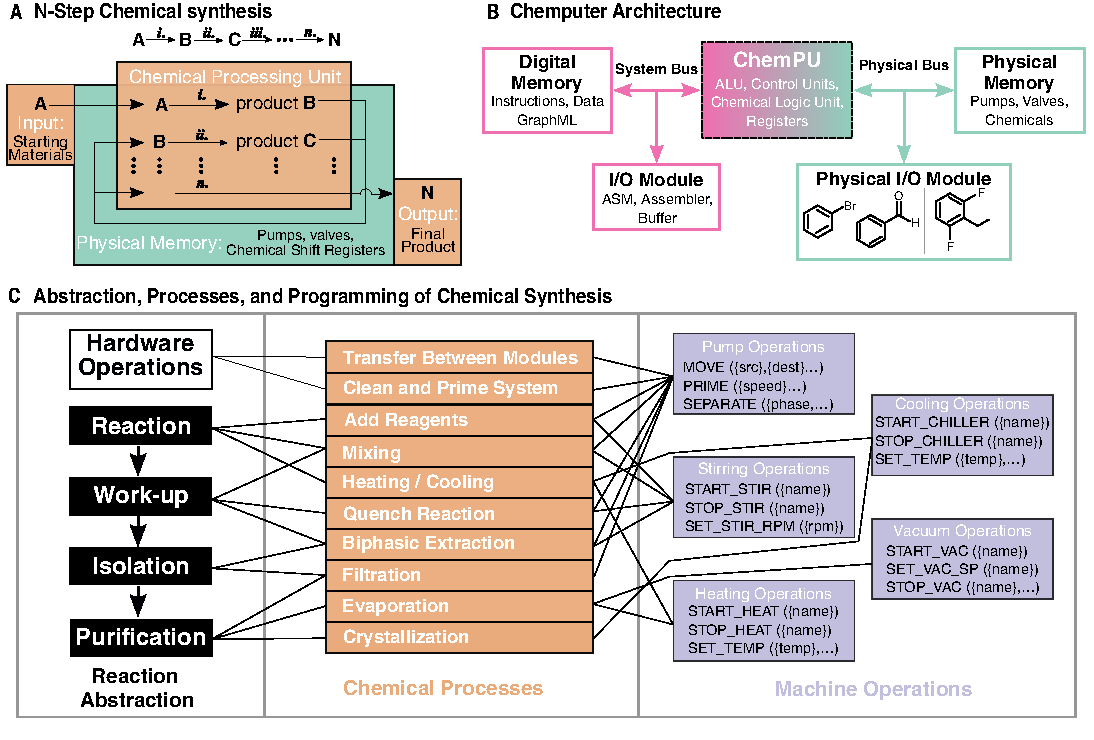
\includegraphics[width=\textwidth,height=0.62\textheight,keepaspectratio]{figures/chapter08-autonomise/04-steiner-chemputer-principles-fig1.pdf}
  \caption{Operating principles of the Chemputer: chemical inputs and operations are abstracted into an executable architecture. Reproduced from Steiner \textit{et al.}, \textit{Science} (2019), Fig.~1.}
  \label{fig8-steiner-principles}
\end{figure}\begin{figure}[htbp]
  \centering
  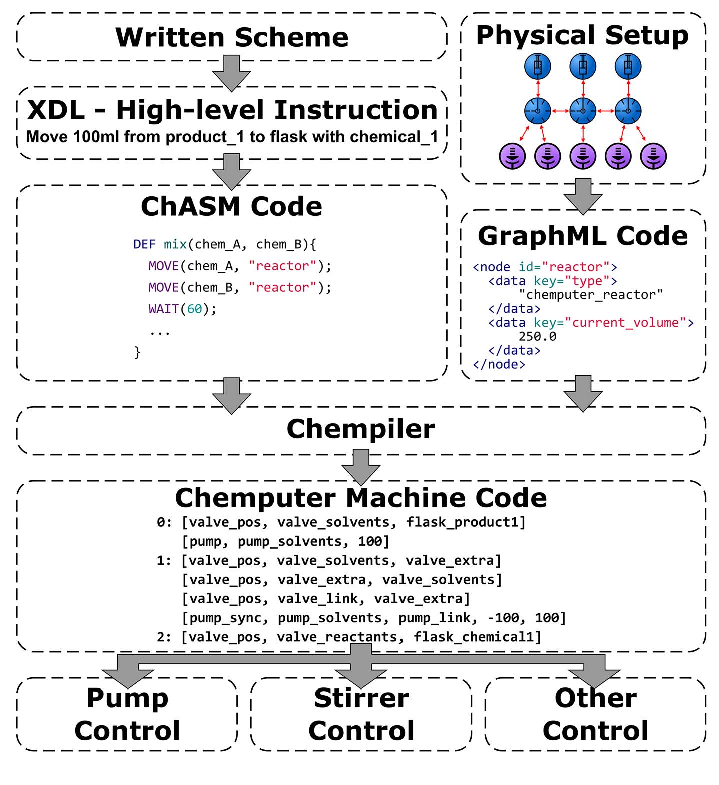
\includegraphics[width=\textwidth,height=0.66\textheight,keepaspectratio]{figures/chapter08-autonomise/05-steiner-information-flow-fig2.pdf}
  \caption{Information flow from written procedure and hardware graph to low-level commands. The procedure is programmable, but the synthetic target and sequence are fixed in advance. Reproduced from Steiner \textit{et al.}, \textit{Science} (2019), Fig.~2.}
  \label{fig8-steiner-flow}
\end{figure}

\solution{4.6cm}{%
  \textbf{Separate representation, compilation, and execution.}
  \begin{itemize}
    \item On Fig.~\ref{fig8-steiner-principles}, mark the chemical procedure, abstraction layer, and physical modules.
    \item On Fig.~\ref{fig8-steiner-flow}, trace one written operation to the pump/valve commands that implement it.
    \item Add the feedback arrow that would be required for autonomy, then state which measurement and decision rule must cross it.
  \end{itemize}
}

\subsection{Autonomy uses measurements to choose subsequent actions}

An autonomous workflow accepts a validated measurement and uses decision logic to select what happens next.
The decision can come from Bayesian optimisation, a classifier, a heuristic rule, or an analytical threshold.
The defining feature is feedback from observed outcome to subsequent experimental action.

\solution{4.2cm}{%
  \begin{tabular}{p{0.24\linewidth}p{0.66\linewidth}}
    \textbf{Automation} & executes a predefined operation or sequence;\\[0.35em]
    \textbf{Programmability} & stores and transfers an executable procedure;\\[0.35em]
    \textbf{Autonomy} & uses measurements to make consequential choices among permitted next actions.
  \end{tabular}
}

\solution{3.8cm}{%
  \textbf{Classify the system.}
  \begin{enumerate}
    \item A liquid handler executes a fixed 384-well screen.
    \item A platform compiles a coded multistep synthesis onto pumps and valves.
    \item A system repeats a reaction if LC quality control fails and advances to scale-up if NMR and MS thresholds pass.
  \end{enumerate}
}

% Suggested timing: 39--47 min
\section{Closed-loop optimisation in physical laboratories}

\subsection{A mobile robotic chemist}

Burger and co-workers used a mobile robot to operate instruments distributed through a conventional laboratory.\mcite{Burger2020}
The robot prepared photocatalyst formulations, transported samples, initiated experiments, and returned measurements to a batched Bayesian search.
Over eight days, it performed 688 experiments in a ten-variable space while searching for improved photocatalysts for hydrogen production from water.

\begin{figure}[htbp]
  \centering
  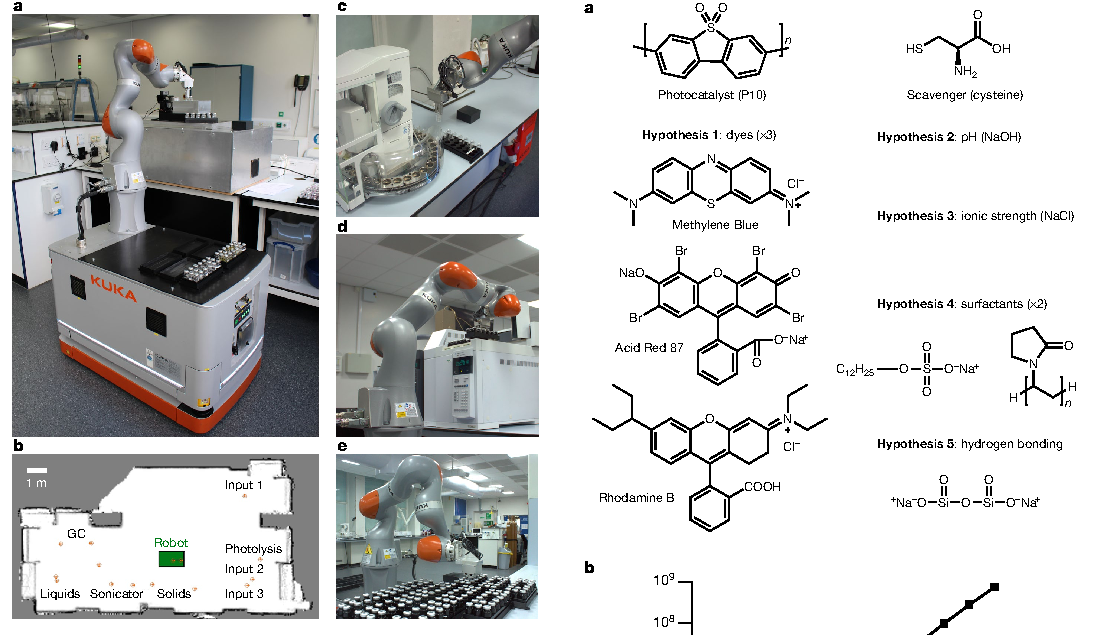
\includegraphics[width=\textwidth,height=0.58\textheight,keepaspectratio]{figures/chapter08-autonomise/06-burger-mobile-robot-platform-fig1.pdf}
  \caption{The mobile robotic chemist operating existing stations in a conventional laboratory. Mobility connects instruments; it does not by itself choose the chemistry. Reproduced from Burger \textit{et al.}, \textit{Nature} (2020), Fig.~1.}
  \label{fig8-burger-platform}
\end{figure}\begin{figure}[htbp]
  \centering
  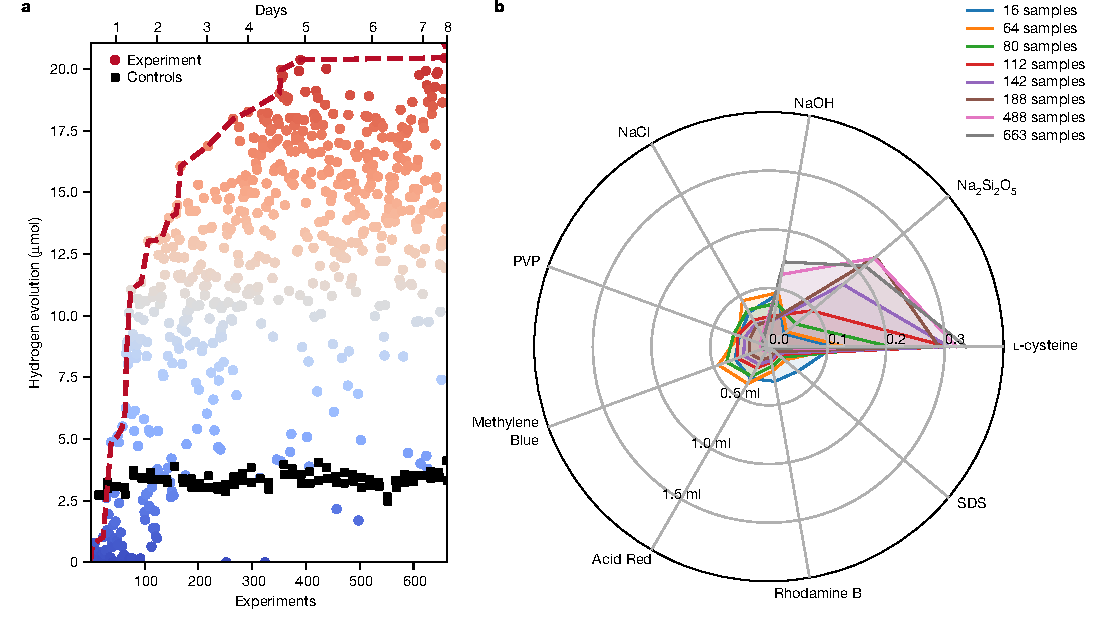
\includegraphics[width=\textwidth,height=0.54\textheight,keepaspectratio]{figures/chapter08-autonomise/07-burger-autonomous-search-output-fig3.pdf}
  \caption{Outcome of the eight-day autonomous search, showing measured hydrogen evolution across the campaign and the robot's movement between stations. Reproduced from Burger \textit{et al.}, \textit{Nature} (2020), Fig.~3.}
  \label{fig8-burger-output}
\end{figure}

The mobile architecture solves an orchestration problem.
Instead of rebuilding every instrument into one enclosed platform, a robotic agent connects equipment that was designed for human use.
The Bayesian search supplies the autonomous element because measured outcomes influence later batches.
Mobility alone would be automation; feedback makes the campaign adaptive.

\solution{3.8cm}{%
  \textbf{Connect the physical platform in Fig.~\ref{fig8-burger-platform} to the search trajectory in Fig.~\ref{fig8-burger-output}.}
  Mark physical transport, experiment execution, measurement, data validation, Bayesian batch selection, and the feedback arrow.
  Circle the stage whose removal would leave an automated but non-autonomous platform.
}

\subsection{RoboChem}

RoboChem integrates flow photochemistry, phase tracking, inline NMR, and Bayesian optimisation in a closed loop.\mcite{Slattery2024}
The platform can optimise mixtures of continuous and categorical variables against yield, productivity, or a combined objective.
Because it operates in a continuous-flow microreactor, optimisation is connected to mass, heat, and photon transport rather than treated as a purely numerical exercise.

\begin{figure}[htbp]
  \centering
  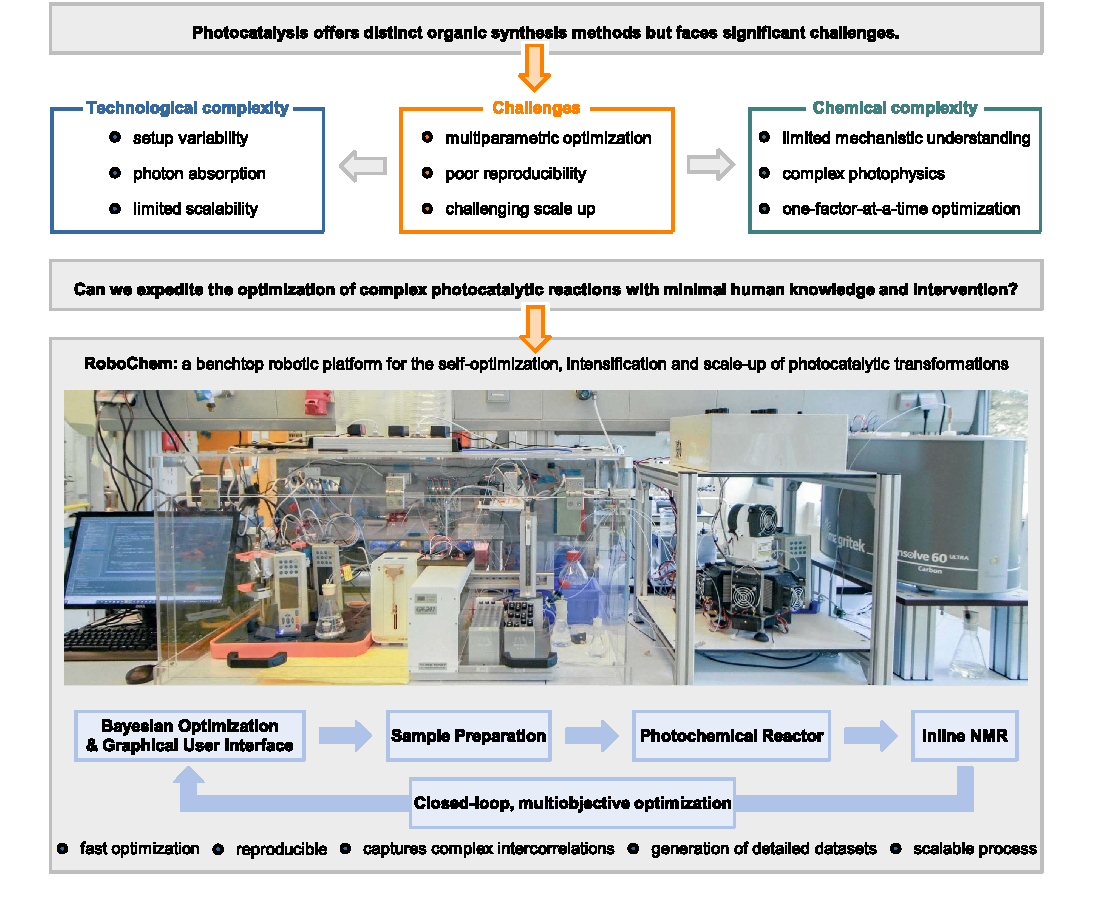
\includegraphics[width=\textwidth,height=0.68\textheight,keepaspectratio]{figures/chapter08-autonomise/08-robochem-closed-loop-concept-fig1.pdf}
  \caption{RoboChem links closed-loop optimisation to replication, intensification, and scale-up in photocatalytic flow chemistry. Reproduced from Slattery \textit{et al.}, \textit{Science} (2024), Fig.~1.}
  \label{fig8-robochem-concept}
\end{figure}

\solution{3.8cm}{%
  \textbf{Before seeing the hardware, label the four claims in the concept figure.}
  \begin{itemize}
    \item optimisation inside the search space;
    \item replication of the selected condition;
    \item intensification of production;
    \item scale-up against a larger material objective.
  \end{itemize}
}\begin{figure}[htbp]
  \centering
  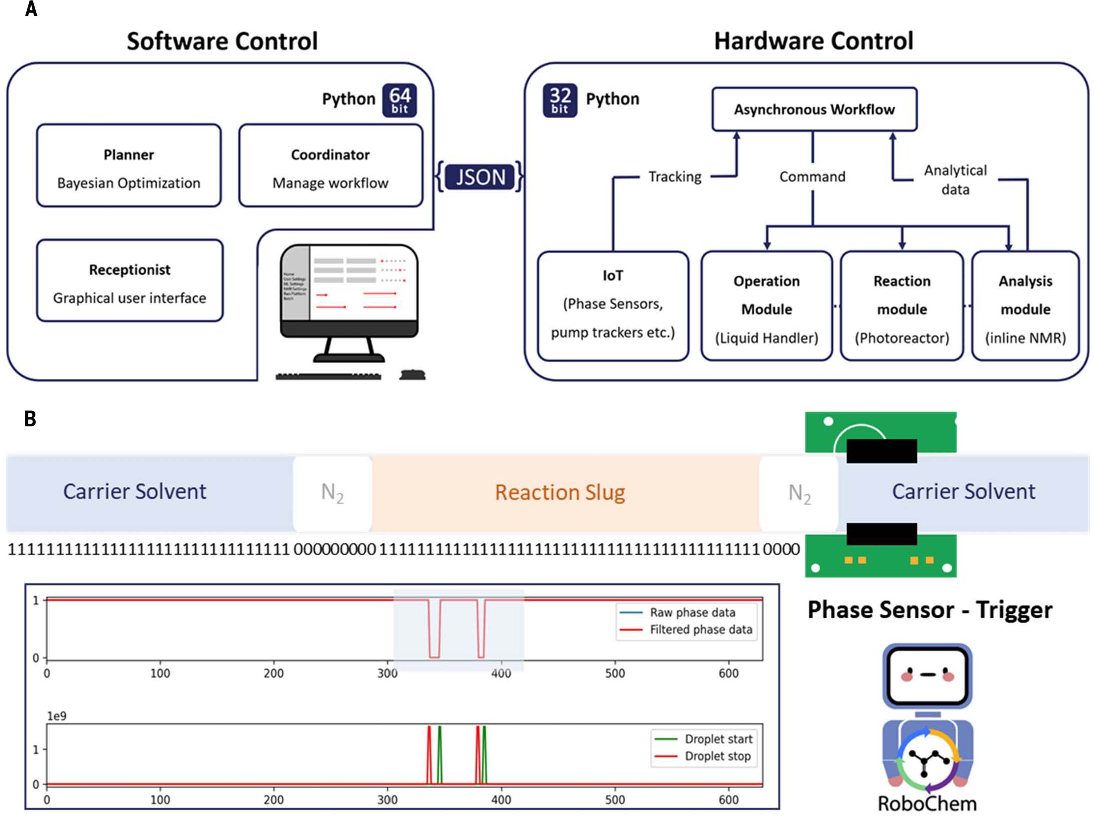
\includegraphics[width=\textwidth,height=0.66\textheight,keepaspectratio]{figures/chapter08-autonomise/09-robochem-platform-architecture-fig2.pdf}
  \caption{RoboChem platform architecture, including reaction-slug tracking, flow photochemistry, inline NMR, and decision software. Reproduced from Slattery \textit{et al.}, \textit{Science} (2024), Fig.~2.}
  \label{fig8-robochem-architecture}
\end{figure}

Optimisation, intensification, and scale-up should remain distinct.
Optimisation identifies favourable conditions inside a defined search space.
Intensification changes how efficiently material is produced.
Scale-up tests whether selected conditions transfer to a larger production objective.
The platform demonstrated these steps across photocatalytic transformations and compared isolated yields with the inline-NMR response.

\begin{figure}[htbp]
  \centering
  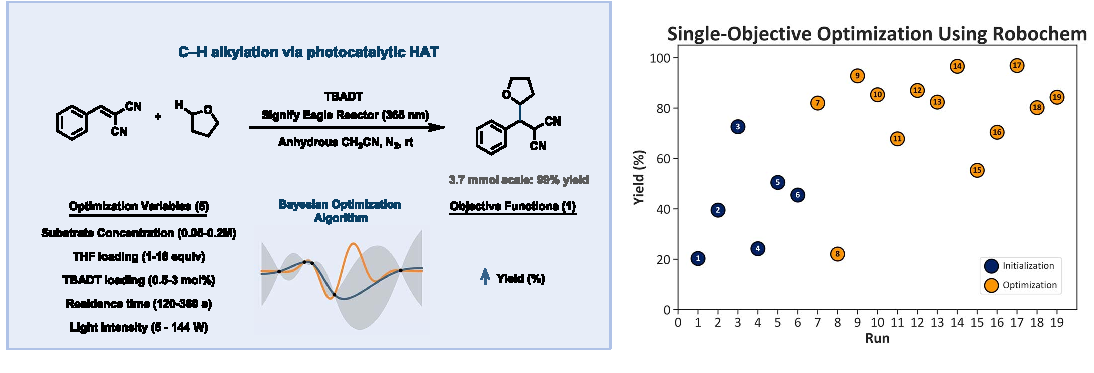
\includegraphics[width=\textwidth,height=0.42\textheight,keepaspectratio]{figures/chapter08-autonomise/10-robochem-optimisation-campaign-fig3.pdf}
  \caption{A representative single-objective RoboChem optimisation campaign. The trajectory is meaningful only together with the defined variables, objective, constraints, and measurement chain. Reproduced from Slattery \textit{et al.}, \textit{Science} (2024), Fig.~3.}
  \label{fig8-robochem-campaign}
\end{figure}

\solution{4.2cm}{%
  \textbf{Annotate Figs.~\ref{fig8-robochem-architecture} and \ref{fig8-robochem-campaign} with three paths:}
  \begin{enumerate}
    \item the material path through the flow reactor;
    \item the information path from NMR to the optimiser and back to conditions;
    \item the transfer from optimisation to intensification and scale-up.
  \end{enumerate}
}

The case also reinforces a lesson from Chapter~7.
A Bayesian optimiser can only learn from the response supplied to it.
Phase tracking, analytical synchronisation, calibration, and valid quality control are part of the optimisation loop, not support services outside it.

% Suggested timing: 47--54 min
\section{Autonomous exploration is not always scalar optimisation}

Dai and co-workers connected an automated synthesiser, UPLC--MS, benchtop NMR, a photoreactor, and other laboratory modules using mobile robots.\mcite{Dai2024}
An application-agnostic planner coordinated the workflow, while application-specific analytical rules determined whether a reaction should be replicated, scaled up, diversified, or passed to a functional host--guest assay.

\begin{figure}[htbp]
  \centering
  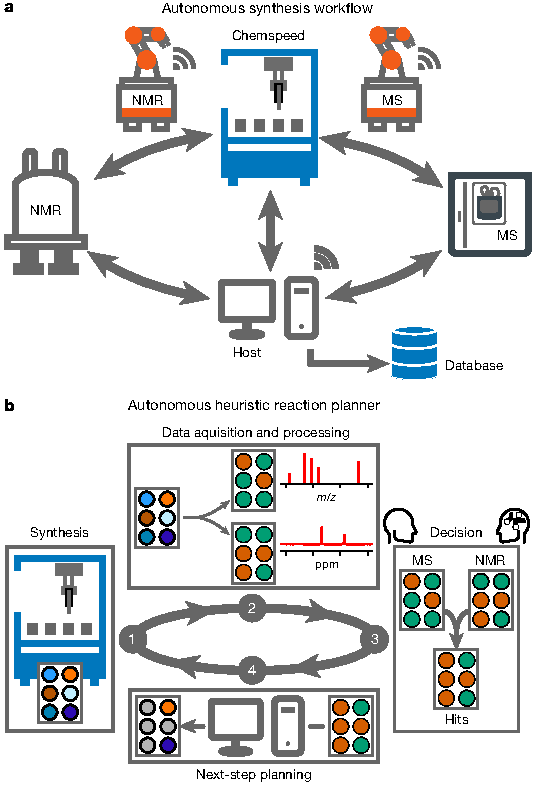
\includegraphics[width=\textwidth,height=0.68\textheight,keepaspectratio]{figures/chapter08-autonomise/11-dai-modular-lab-planner-fig1.pdf}
  \caption{Modular mobile-robot laboratory and heuristic reaction planner. Orthogonal analytical measurements determine which branches are permitted next. Reproduced from Dai \textit{et al.}, \textit{Nature} (2024), Fig.~1.}
  \label{fig8-dai-planner}
\end{figure}

\solution{4.2cm}{%
  \textbf{Trace material and evidence separately.}
  \begin{itemize}
    \item Draw the material path among synthesis, UPLC--MS, and NMR stations.
    \item Draw the information path from both analyses to the planner.
    \item Mark which decisions are application-agnostic orchestration and which require application-specific thresholds.
  \end{itemize}
}

These workflows are autonomous because measurements determine subsequent actions.
They are not all closed-loop optimisations of one scalar response.
Exploratory chemistry often branches among qualitatively different decisions: Is the proposed product present? Is the result reproducible? Is there enough material for characterisation? Should related reactions be explored? Does the product perform a function?

\begin{figure}[htbp]
  \centering
  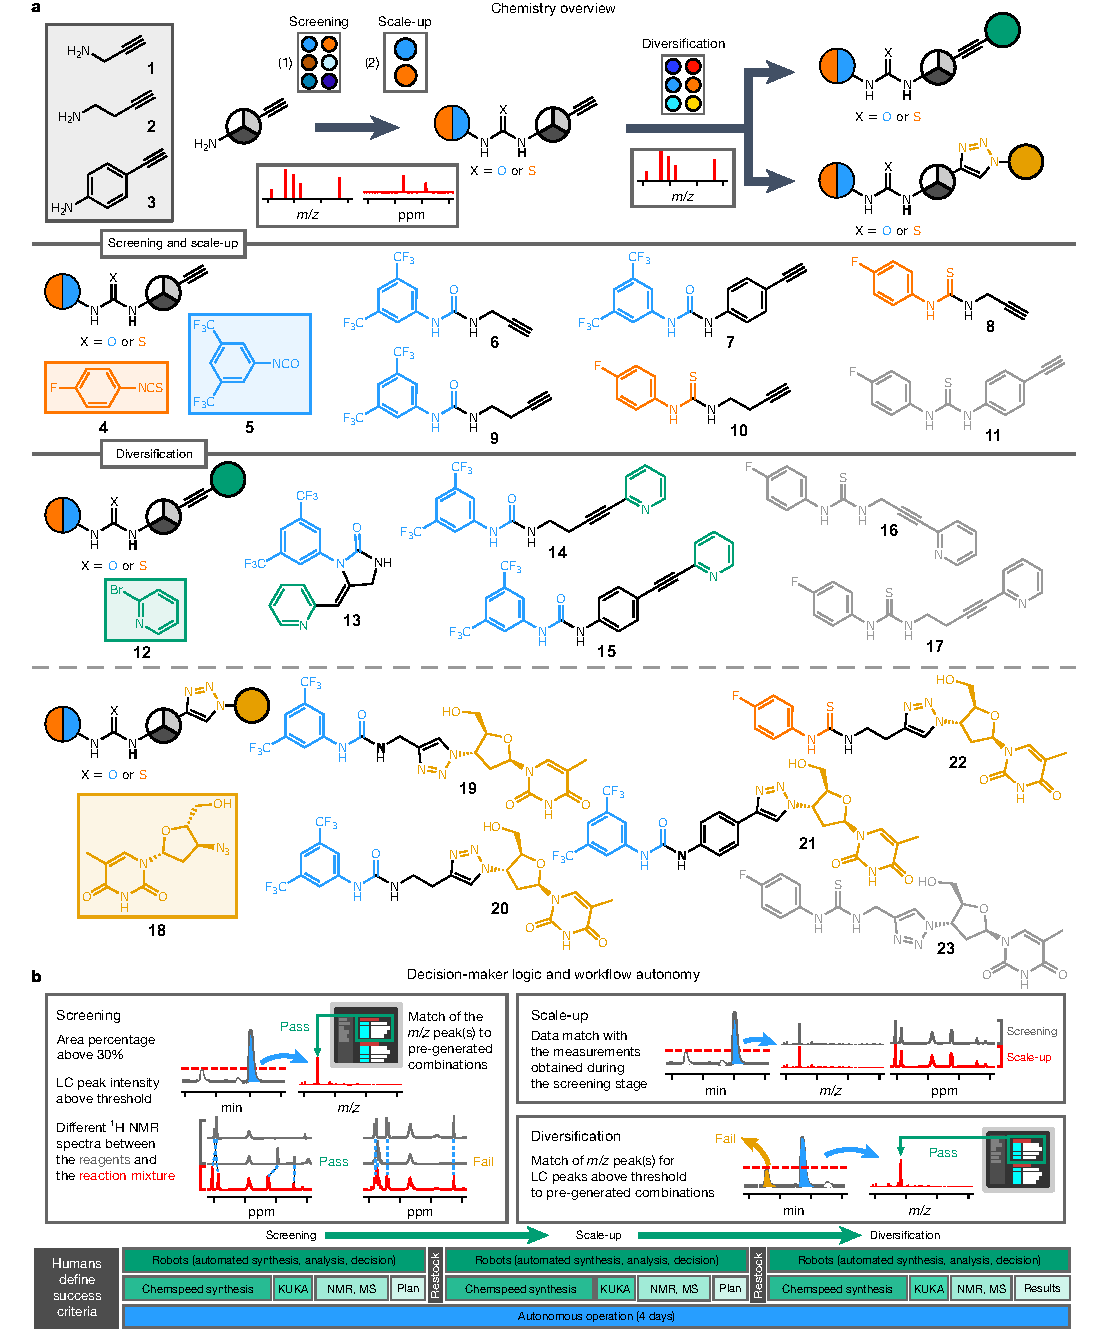
\includegraphics[width=\textwidth,height=0.72\textheight,keepaspectratio]{figures/chapter08-autonomise/12-dai-divergent-synthesis-fig2.pdf}
  \caption{Autonomous divergent synthesis and the heuristic logic for screening, replication, scale-up, and diversification. Reproduced from Dai \textit{et al.}, \textit{Nature} (2024), Fig.~2.}
  \label{fig8-dai-divergent}
\end{figure}

\solution{4.5cm}{%
  \textbf{Annotate one complete branch from proposal to decision.}
  \begin{itemize}
    \item Mark the analytical threshold that permits replication.
    \item Mark the evidence required before scale-up or diversification.
    \item Circle a failed branch and distinguish chemical failure from analytical or execution failure.
    \item Add the point at which a human should inspect an unexpected product.
  \end{itemize}
}

Orthogonal analysis matters because one measurement can be ambiguous.
A mass consistent with a target does not prove connectivity.
An NMR signal can support symmetry or conversion but may not identify every species.
The workflow required combinations of analytical evidence to pass predefined thresholds before advancing.

\begin{figure}[htbp]
  \centering
  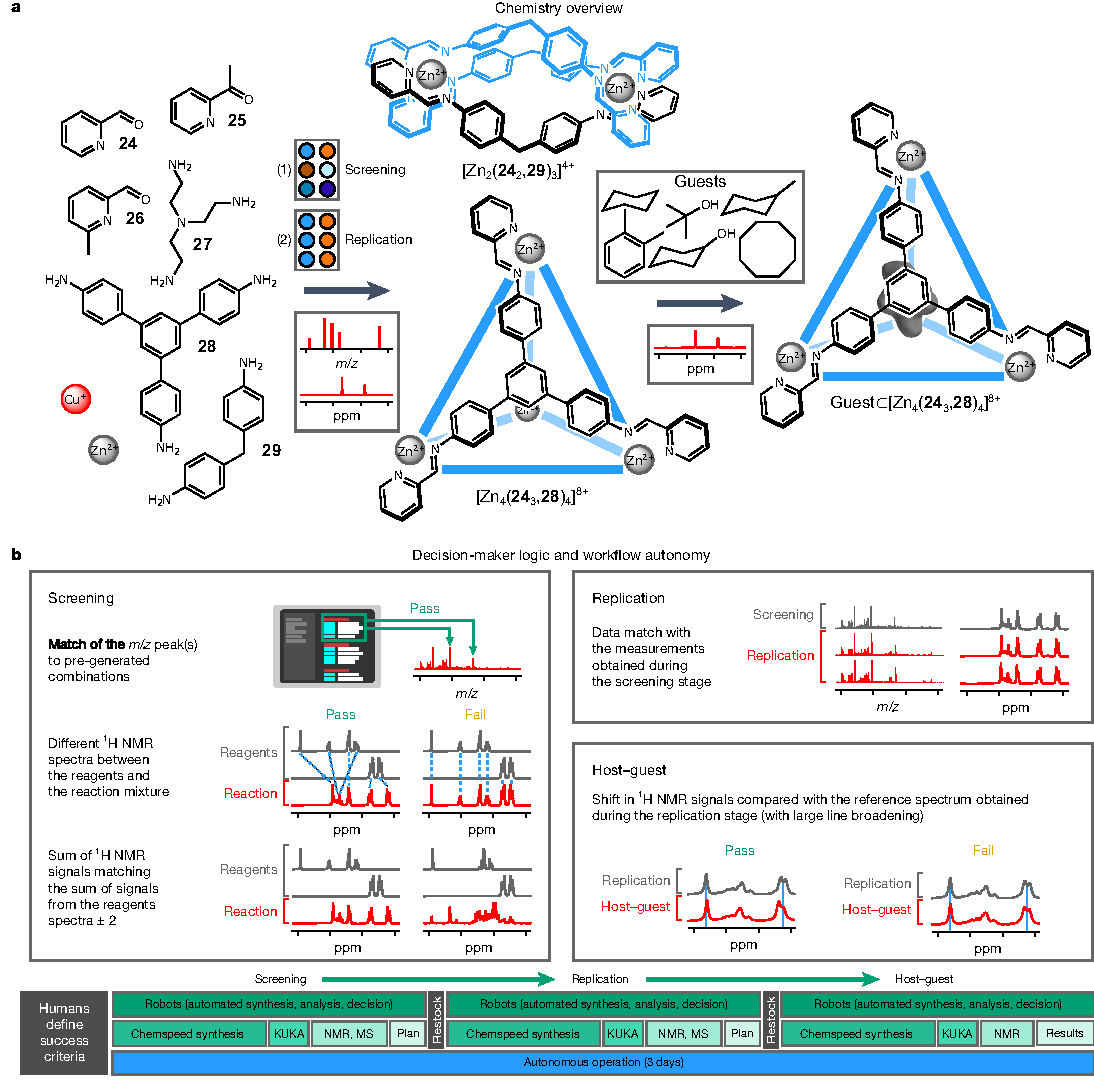
\includegraphics[width=\textwidth,height=0.72\textheight,keepaspectratio]{figures/chapter08-autonomise/13-dai-host-guest-discovery-fig3.pdf}
  \caption{Autonomous supramolecular host--guest exploration using combinations of components and analytical decision rules. The workflow branches on evidence rather than maximising one scalar response. Reproduced from Dai \textit{et al.}, \textit{Nature} (2024), Fig.~3.}
  \label{fig8-dai-hostguest}
\end{figure}

\solution{4.5cm}{%
  \textbf{Read the host--guest workflow as a chain of claims.}
  \begin{itemize}
    \item Mark what MS supports and what it cannot establish alone.
    \item Mark what NMR contributes to composition, symmetry, or binding evidence.
    \item Identify the threshold that advances a candidate to the functional assay.
    \item Write one plausible host--guest interpretation that would still require human chemical judgement.
  \end{itemize}
}

The study also exposed the limit of encoded context.
An unexpected cyclisation was not recognised by the initial UPLC--MS decision rule and required later human interpretation.
The platform acted consistently with the evidence and thresholds it had been given; the missing chemical interpretation lay outside that representation.

\solution{4.5cm}{%
  \textbf{Draw a branching decision tree.}
  \begin{itemize}
    \item UPLC--MS fails quality control $\rightarrow$ repeat or diagnose;
    \item mass and NMR criteria pass $\rightarrow$ replicate;
    \item replication succeeds $\rightarrow$ scale up or diversify;
    \item sufficient material and identity evidence $\rightarrow$ functional assay;
    \item ambiguous or unexpected data $\rightarrow$ human review.
  \end{itemize}
}

\begin{conceptbox}
  \keypoint{Autonomous does not necessarily mean optimising.}
  A system can make consequential experimental choices through rules, thresholds, and branching logic without repeatedly fitting a scalar objective model.
\end{conceptbox}

% Suggested timing: 54--58 min
\section{A self-driving loop must survive failure}

A closed-loop platform must distinguish a chemical negative result from hardware, execution, analytical, and processing failures.
A blocked line, empty reagent bottle, missed injection, detector drift, saturated signal, failed integration, and genuinely inactive reaction require different responses.

Quality-control logic should determine whether a result is accepted, repeated, diagnosed, or escalated.
Safe recovery can include inventory tracking, pressure and temperature limits, instrument watchdogs, calibration checks, bounded retries, and a defined shutdown state.
Every rejected or repeated experiment should retain a traceable reason.
Otherwise a later model may treat a fault-generated value as chemistry.

\solution{4.5cm}{%
  \textbf{Design the response to four events.}
  \begin{enumerate}
    \item no product detected, with all controls valid;
    \item no analytical injection recorded;
    \item reactor pressure exceeds its limit;
    \item repeated model recommendations approach an insoluble region.
  \end{enumerate}
  Label each response as accept, repeat, diagnose, constrain, escalate, or shut down.
}

A self-driving laboratory therefore needs a state richer than a table of objective values.
It needs quality flags, equipment state, reagent inventory, procedural provenance, constraints, and decision history.
Scientific auditability requires reconstructing why an experiment was selected and which evidence caused the next action.

% Suggested timing: 58--60 min
\section{Human responsibility and the delegated decision space}

Humans define the chemical problem, objective, constraints, permitted actions, evidence required for success, and conditions for intervention.
The autonomous system chooses only inside that delegated decision space.

An objective that rewards yield alone can direct a platform towards expensive, hazardous, or wasteful conditions unless those consequences appear as constraints or additional objectives.
A system that cannot represent a mechanistic change cannot be expected to diagnose it reliably.
A system that receives only one analytical signal cannot reason with evidence that was never measured.

\solution{3.5cm}{%
  \textbf{For one proposed autonomous campaign, state:}
  \begin{itemize}
    \item what the system may choose;
    \item what it may never choose;
    \item which evidence permits automatic progression;
    \item which events require human interpretation;
    \item how the complete decision history will be audited.
  \end{itemize}
}

\section{Closing the course}

The course began by translating molecular structures into representations that computers can store and compare.
Descriptors then placed molecules in chemical spaces.
Models connected those representations to measured responses.
Validation asked which new chemistry those relationships could support.
Experimental design and automation generated consistent, information-rich data.
Sequential selection used those measurements to choose subsequent actions.

\solution{4.0cm}{%
  \centering
  represent $\longrightarrow$ model $\longrightarrow$ select $\longrightarrow$ execute\\[0.6em]
  $\longrightarrow$ measure $\longrightarrow$ validate $\longrightarrow$ update\\[0.6em]
  $\longrightarrow$ select again
}

Every stage inherits limitations from the earlier stages.
A poor representation hides relevant chemistry.
A narrow dataset limits transfer.
An inappropriate objective rewards the wrong outcome.
An unreliable measurement corrupts the feedback signal.
A decision rule without failure handling converts instrument faults into scientific conclusions.

A self-driving laboratory is therefore not one robot or one optimisation algorithm.
It is a validated relationship among a chemical objective, a defined candidate space, executable operations, trustworthy measurements, explicit decision logic, constraints, provenance, and safe recovery.

\section{Summary}

Fixed design chooses experiments before outcomes are known; sequential design allows measurements to alter later choices.
Bayesian optimisation combines a surrogate model with an acquisition function that balances exploration and exploitation.
The Shields study shows the value and bounded nature of Bayesian reaction optimisation under a fixed budget.
Pareto fronts expose multiobjective trade-offs but do not choose values on behalf of the chemist.
Automated peptide synthesis demonstrates predefined repetitive execution, while the Chemputer demonstrates transferable programmable procedures.
The mobile robotic chemist and RoboChem connect physical execution with measured feedback and adaptive optimisation.
The Dai platform demonstrates autonomous branching for exploratory synthesis without reducing discovery to one scalar objective.
Robust autonomy depends on quality control, explicit failure states, constraints, recovery, auditability, and a clearly defined role for human judgement.
